\subsection{Pruebas y resultados}
	A continuación se muestran los resultados obtenidos para 2x2.


	Primeramente, se muestran dos archivos obtenidos como resultado de ejecutar el programa arboles.py, como se puede observar en ambos casos, el archivo ya se encuentra acomodado para ser usado con Mermaid.cli.


	\paragraph{Archivo generado:} tam-2-life.mmd
	\lstinputlisting[language=Java]{../../Arboles/tam-2-life.mmd}
	
	\paragraph{Archivo generado:} tam-2-diffusion.mmd:
	\lstinputlisting[language=Java]{../../Arboles/tam-2-diffusion.mmd}

	Posteriormente, las figuras \ref{fig:graf1} y \ref{fig:graf2} muestran los arboles obtenidos después de usar los archivos anteriormente mostrados con Mermaid.cli.

	\begin{figure}[H]
		\begin{center}
			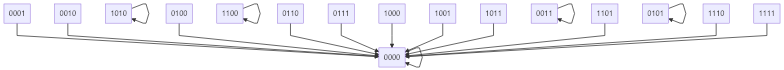
\includegraphics[scale=.5]{Grafos/img/tam-2-life.png}
			\caption{Árbol obtenido para 2x2 Life}
			\label{fig:graf1}
		\end{center}
	\end{figure}

	\begin{figure}[H]
		\begin{center}
			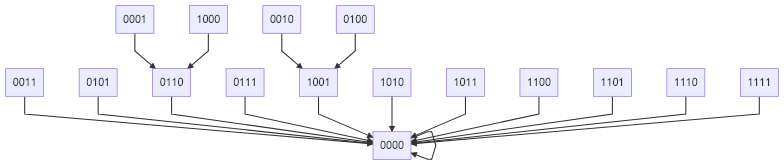
\includegraphics[scale=.5]{Grafos/img/tam-2-diffusion.png}
			\caption{Árbol obtenido para 2x2 Difusión}
			\label{fig:graf2}
		\end{center}
	\end{figure}